
%% bare_jrnl_compsoc.tex
%% V1.4b
%% 2015/08/26
%% by Michael Shell
%% See:
%% http://www.michaelshell.org/
%% for current contact information.
%%
%% This is a skeleton file demonstrating the use of IEEEtran.cls
%% (requires IEEEtran.cls version 1.8b or later) with an IEEE
%% Computer Society journal paper.
%%
%% Support sites:
%% http://www.michaelshell.org/tex/ieeetran/
%% http://www.ctan.org/pkg/ieeetran
%% and
%% http://www.ieee.org/

%%*************************************************************************
%% Legal Notice:
%% This code is offered as-is without any warranty either expressed or
%% implied; without even the implied warranty of MERCHANTABILITY or
%% FITNESS FOR A PARTICULAR PURPOSE! 
%% User assumes all risk.
%% In no event shall the IEEE or any contributor to this code be liable for
%% any damages or losses, including, but not limited to, incidental,
%% consequential, or any other damages, resulting from the use or misuse
%% of any information contained here.
%%
%% All comments are the opinions of their respective authors and are not
%% necessarily endorsed by the IEEE.
%%
%% This work is distributed under the LaTeX Project Public License (LPPL)
%% ( http://www.latex-project.org/ ) version 1.3, and may be freely used,
%% distributed and modified. A copy of the LPPL, version 1.3, is included
%% in the base LaTeX documentation of all distributions of LaTeX released
%% 2003/12/01 or later.
%% Retain all contribution notices and credits.
%% ** Modified files should be clearly indicated as such, including  **
%% ** renaming them and changing author support contact information. **
%%*************************************************************************


% *** Authors should verify (and, if needed, correct) their LaTeX system  ***
% *** with the testflow diagnostic prior to trusting their LaTeX platform ***
% *** with production work. The IEEE's font choices and paper sizes can   ***
% *** trigger bugs that do not appear when using other class files.       ***                          ***
% The testflow support page is at:
% http://www.michaelshell.org/tex/testflow/


\documentclass[10pt,journal,compsoc]{IEEEtran}
%
% If IEEEtran.cls has not been installed into the LaTeX system files,
% manually specify the path to it like:
% \documentclass[10pt,journal,compsoc]{../sty/IEEEtran}



\usepackage{hyperref}

\usepackage{listings}
\usepackage{framed}

\usepackage{amsmath,amssymb,booktabs}
% Some very useful LaTeX packages include:
% (uncomment the ones you want to load)

\usepackage{tikz}
\usepackage{pgf-umlsd}
\usepgflibrary{arrows}
\usepackage[algo2e]{algorithm2e}
\usepackage{multicol}

\newcommand\tabhead[1]{\small\textbf{#1}}
% *** MISC UTILITY PACKAGES ***
%
%\usepackage{ifpdf}
% Heiko Oberdiek's ifpdf.sty is very useful if you need conditional
% compilation based on whether the output is pdf or dvi.
% usage:
% \ifpdf
%   % pdf code
% \else
%   % dvi code
% \fi
% The latest version of ifpdf.sty can be obtained from:
% http://www.ctan.org/pkg/ifpdf
% Also, note that IEEEtran.cls V1.7 and later provides a builtin
% \ifCLASSINFOpdf conditional that works the same way.
% When switching from latex to pdflatex and vice-versa, the compiler may
% have to be run twice to clear warning/error messages.






% *** CITATION PACKAGES ***
%
\ifCLASSOPTIONcompsoc
  % IEEE Computer Society needs nocompress option
  % requires cite.sty v4.0 or later (November 2003)
  \usepackage[nocompress]{cite}
\else
  % normal IEEE
  \usepackage{cite}
\fi
% cite.sty was written by Donald Arseneau
% V1.6 and later of IEEEtran pre-defines the format of the cite.sty package
% \cite{} output to follow that of the IEEE. Loading the cite package will
% result in citation numbers being automatically sorted and properly
% "compressed/ranged". e.g., [1], [9], [2], [7], [5], [6] without using
% cite.sty will become [1], [2], [5]--[7], [9] using cite.sty. cite.sty's
% \cite will automatically add leading space, if needed. Use cite.sty's
% noadjust option (cite.sty V3.8 and later) if you want to turn this off
% such as if a citation ever needs to be enclosed in parenthesis.
% cite.sty is already installed on most LaTeX systems. Be sure and use
% version 5.0 (2009-03-20) and later if using hyperref.sty.
% The latest version can be obtained at:
% http://www.ctan.org/pkg/cite
% The documentation is contained in the cite.sty file itself.
%
% Note that some packages require special options to format as the Computer
% Society requires. In particular, Computer Society  papers do not use
% compressed citation ranges as is done in typical IEEE papers
% (e.g., [1]-[4]). Instead, they list every citation separately in order
% (e.g., [1], [2], [3], [4]). To get the latter we need to load the cite
% package with the nocompress option which is supported by cite.sty v4.0
% and later. Note also the use of a CLASSOPTION conditional provided by
% IEEEtran.cls V1.7 and later.





% *** GRAPHICS RELATED PACKAGES ***
%
\ifCLASSINFOpdf
  %\usepackage[pdftex]{graphicx}
  % declare the path(s) where your graphic files are
  % \graphicspath{{../pdf/}{../jpeg/}}
  % and their extensions so you won't have to specify these with
  % every instance of \includegraphics
  % \DeclareGraphicsExtensions{.pdf,.jpeg,.png}
\else
  % or other class option (dvipsone, dvipdf, if not using dvips). graphicx
  % will default to the driver specified in the system graphics.cfg if no
  % driver is specified.
  % \usepackage[dvips]{graphicx}
  % declare the path(s) where your graphic files are
  % \graphicspath{{../eps/}}
  % and their extensions so you won't have to specify these with
  % every instance of \includegraphics
  % \DeclareGraphicsExtensions{.eps}
\fi
% graphicx was written by David Carlisle and Sebastian Rahtz. It is
% required if you want graphics, photos, etc. graphicx.sty is already
% installed on most LaTeX systems. The latest version and documentation
% can be obtained at: 
% http://www.ctan.org/pkg/graphicx
% Another good source of documentation is "Using Imported Graphics in
% LaTeX2e" by Keith Reckdahl which can be found at:
% http://www.ctan.org/pkg/epslatex
%
% latex, and pdflatex in dvi mode, support graphics in encapsulated
% postscript (.eps) format. pdflatex in pdf mode supports graphics
% in .pdf, .jpeg, .png and .mps (metapost) formats. Users should ensure
% that all non-photo figures use a vector format (.eps, .pdf, .mps) and
% not a bitmapped formats (.jpeg, .png). The IEEE frowns on bitmapped formats
% which can result in "jaggedy"/blurry rendering of lines and letters as
% well as large increases in file sizes.
%
% You can find documentation about the pdfTeX application at:
% http://www.tug.org/applications/pdftex






% *** MATH PACKAGES ***
%
%\usepackage{amsmath}
% A popular package from the American Mathematical Society that provides
% many useful and powerful commands for dealing with mathematics.
%
% Note that the amsmath package sets \interdisplaylinepenalty to 10000
% thus preventing page breaks from occurring within multiline equations. Use:
%\interdisplaylinepenalty=2500
% after loading amsmath to restore such page breaks as IEEEtran.cls normally
% does. amsmath.sty is already installed on most LaTeX systems. The latest
% version and documentation can be obtained at:
% http://www.ctan.org/pkg/amsmath





% *** SPECIALIZED LIST PACKAGES ***
%
%\usepackage{algorithmic}
% algorithmic.sty was written by Peter Williams and Rogerio Brito.
% This package provides an algorithmic environment fo describing algorithms.
% You can use the algorithmic environment in-text or within a figure
% environment to provide for a floating algorithm. Do NOT use the algorithm
% floating environment provided by algorithm.sty (by the same authors) or
% algorithm2e.sty (by Christophe Fiorio) as the IEEE does not use dedicated
% algorithm float types and packages that provide these will not provide
% correct IEEE style captions. The latest version and documentation of
% algorithmic.sty can be obtained at:
% http://www.ctan.org/pkg/algorithms
% Also of interest may be the (relatively newer and more customizable)
% algorithmicx.sty package by Szasz Janos:
% http://www.ctan.org/pkg/algorithmicx




% *** ALIGNMENT PACKAGES ***
%
%\usepackage{array}
% Frank Mittelbach's and David Carlisle's array.sty patches and improves
% the standard LaTeX2e array and tabular environments to provide better
% appearance and additional user controls. As the default LaTeX2e table
% generation code is lacking to the point of almost being broken with
% respect to the quality of the end results, all users are strongly
% advised to use an enhanced (at the very least that provided by array.sty)
% set of table tools. array.sty is already installed on most systems. The
% latest version and documentation can be obtained at:
% http://www.ctan.org/pkg/array


% IEEEtran contains the IEEEeqnarray family of commands that can be used to
% generate multiline equations as well as matrices, tables, etc., of high
% quality.




% *** SUBFIGURE PACKAGES ***
\ifCLASSOPTIONcompsoc
  \usepackage[caption=false,font=footnotesize,labelfont=sf,textfont=sf]{subfig}
\else
  \usepackage[caption=false,font=footnotesize]{subfig}
\fi
% subfig.sty, written by Steven Douglas Cochran, is the modern replacement
% for subfigure.sty, the latter of which is no longer maintained and is
% incompatible with some LaTeX packages including fixltx2e. However,
% subfig.sty requires and automatically loads Axel Sommerfeldt's caption.sty
% which will override IEEEtran.cls' handling of captions and this will result
% in non-IEEE style figure/table captions. To prevent this problem, be sure
% and invoke subfig.sty's "caption=false" package option (available since
% subfig.sty version 1.3, 2005/06/28) as this is will preserve IEEEtran.cls
% handling of captions.
% Note that the Computer Society format requires a sans serif font rather
% than the serif font used in traditional IEEE formatting and thus the need
% to invoke different subfig.sty package options depending on whether
% compsoc mode has been enabled.
%
% The latest version and documentation of subfig.sty can be obtained at:
% http://www.ctan.org/pkg/subfig




% *** FLOAT PACKAGES ***
%
%\usepackage{fixltx2e}
% fixltx2e, the successor to the earlier fix2col.sty, was written by
% Frank Mittelbach and David Carlisle. This package corrects a few problems
% in the LaTeX2e kernel, the most notable of which is that in current
% LaTeX2e releases, the ordering of single and double column floats is not
% guaranteed to be preserved. Thus, an unpatched LaTeX2e can allow a
% single column figure to be placed prior to an earlier double column
% figure.
% Be aware that LaTeX2e kernels dated 2015 and later have fixltx2e.sty's
% corrections already built into the system in which case a warning will
% be issued if an attempt is made to load fixltx2e.sty as it is no longer
% needed.
% The latest version and documentation can be found at:
% http://www.ctan.org/pkg/fixltx2e


%\usepackage{stfloats}
% stfloats.sty was written by Sigitas Tolusis. This package gives LaTeX2e
% the ability to do double column floats at the bottom of the page as well
% as the top. (e.g., "\begin{figure*}[!b]" is not normally possible in
% LaTeX2e). It also provides a command:
%\fnbelowfloat
% to enable the placement of footnotes below bottom floats (the standard
% LaTeX2e kernel puts them above bottom floats). This is an invasive package
% which rewrites many portions of the LaTeX2e float routines. It may not work
% with other packages that modify the LaTeX2e float routines. The latest
% version and documentation can be obtained at:
% http://www.ctan.org/pkg/stfloats
% Do not use the stfloats baselinefloat ability as the IEEE does not allow
% \baselineskip to stretch. Authors submitting work to the IEEE should note
% that the IEEE rarely uses double column equations and that authors should try
% to avoid such use. Do not be tempted to use the cuted.sty or midfloat.sty
% packages (also by Sigitas Tolusis) as the IEEE does not format its papers in
% such ways.
% Do not attempt to use stfloats with fixltx2e as they are incompatible.
% Instead, use Morten Hogholm'a dblfloatfix which combines the features
% of both fixltx2e and stfloats:
%
% \usepackage{dblfloatfix}
% The latest version can be found at:
% http://www.ctan.org/pkg/dblfloatfix




%\ifCLASSOPTIONcaptionsoff
%  \usepackage[nomarkers]{endfloat}
% \let\MYoriglatexcaption\caption
% \renewcommand{\caption}[2][\relax]{\MYoriglatexcaption[#2]{#2}}
%\fi
% endfloat.sty was written by James Darrell McCauley, Jeff Goldberg and 
% Axel Sommerfeldt. This package may be useful when used in conjunction with 
% IEEEtran.cls'  captionsoff option. Some IEEE journals/societies require that
% submissions have lists of figures/tables at the end of the paper and that
% figures/tables without any captions are placed on a page by themselves at
% the end of the document. If needed, the draftcls IEEEtran class option or
% \CLASSINPUTbaselinestretch interface can be used to increase the line
% spacing as well. Be sure and use the nomarkers option of endfloat to
% prevent endfloat from "marking" where the figures would have been placed
% in the text. The two hack lines of code above are a slight modification of
% that suggested by in the endfloat docs (section 8.4.1) to ensure that
% the full captions always appear in the list of figures/tables - even if
% the user used the short optional argument of \caption[]{}.
% IEEE papers do not typically make use of \caption[]'s optional argument,
% so this should not be an issue. A similar trick can be used to disable
% captions of packages such as subfig.sty that lack options to turn off
% the subcaptions:
% For subfig.sty:
% \let\MYorigsubfloat\subfloat
% \renewcommand{\subfloat}[2][\relax]{\MYorigsubfloat[]{#2}}
% However, the above trick will not work if both optional arguments of
% the \subfloat command are used. Furthermore, there needs to be a
% description of each subfigure *somewhere* and endfloat does not add
% subfigure captions to its list of figures. Thus, the best approach is to
% avoid the use of subfigure captions (many IEEE journals avoid them anyway)
% and instead reference/explain all the subfigures within the main caption.
% The latest version of endfloat.sty and its documentation can obtained at:
% http://www.ctan.org/pkg/endfloat
%
% The IEEEtran \ifCLASSOPTIONcaptionsoff conditional can also be used
% later in the document, say, to conditionally put the References on a 
% page by themselves.




% *** PDF, URL AND HYPERLINK PACKAGES ***
%
\usepackage{url}
% url.sty was written by Donald Arseneau. It provides better support for
% handling and breaking URLs. url.sty is already installed on most LaTeX
% systems. The latest version and documentation can be obtained at:
% http://www.ctan.org/pkg/url
% Basically, \url{my_url_here}.





% *** Do not adjust lengths that control margins, column widths, etc. ***
% *** Do not use packages that alter fonts (such as pslatex).         ***
% There should be no need to do such things with IEEEtran.cls V1.6 and later.
% (Unless specifically asked to do so by the journal or conference you plan
% to submit to, of course. )


% correct bad hyphenation here
\hyphenation{op-tical net-works semi-conduc-tor}


\begin{document}
%
% paper title
% Titles are generally capitalized except for words such as a, an, and, as,
% at, but, by, for, in, nor, of, on, or, the, to and up, which are usually
% not capitalized unless they are the first or last word of the title.
% Linebreaks \\ can be used within to get better formatting as desired.
% Do not put math or special symbols in the title.
\title{Incentivizing global crowdsensing with mediated Bitcoin micropayment channels}
%
%
% author names and IEEE memberships
% note positions of commas and nonbreaking spaces ( ~ ) LaTeX will not break
% a structure at a ~ so this keeps an author's name from being broken across
% two lines.
% use \thanks{} to gain access to the first footnote area
% a separate \thanks must be used for each paragraph as LaTeX2e's \thanks
% was not built to handle multiple paragraphs
%
%
%\IEEEcompsocitemizethanks is a special \thanks that produces the bulleted
% lists the Computer Society journals use for "first footnote" author
% affiliations. Use \IEEEcompsocthanksitem which works much like \item
% for each affiliation group. When not in compsoc mode,
% \IEEEcompsocitemizethanks becomes like \thanks and
% \IEEEcompsocthanksitem becomes a line break with idention. This
% facilitates dual compilation, although admittedly the differences in the
% desired content of \author between the different types of papers makes a
% one-size-fits-all approach a daunting prospect. For instance, compsoc 
% journal papers have the author affiliations above the "Manuscript
% received ..."  text while in non-compsoc journals this is reversed. Sigh.

% \author{Michael~Shell,~\IEEEmembership{Member,~IEEE,}
%         John~Doe,~\IEEEmembership{Fellow,~OSA,}
%         and~Jane~Doe,~\IEEEmembership{Life~Fellow,~IEEE}% <-this % stops a space
% \IEEEcompsocitemizethanks{\IEEEcompsocthanksitem M. Shell was with the Department
% of Electrical and Computer Engineering, Georgia Institute of Technology, Atlanta,
% GA, 30332.\protect\\
% % note need leading \protect in front of \\ to get a newline within \thanks as
% % \\ is fragile and will error, could use \hfil\break instead.
% E-mail: see http://www.michaelshell.org/contact.html
% \IEEEcompsocthanksitem J. Doe and J. Doe are with Anonymous University.}% <-this % stops an unwanted space
% \thanks{Manuscript received April 19, 2005; revised August 26, 2015.}}

% note the % following the last \IEEEmembership and also \thanks - 
% these prevent an unwanted space from occurring between the last author name
% and the end of the author line. i.e., if you had this:
% 
% \author{....lastname \thanks{...} \thanks{...} }
%                     ^------------^------------^----Do not want these spaces!
%
% a space would be appended to the last name and could cause every name on that
% line to be shifted left slightly. This is one of those "LaTeX things". For
% instance, "\textbf{A} \textbf{B}" will typeset as "A B" not "AB". To get
% "AB" then you have to do: "\textbf{A}\textbf{B}"
% \thanks is no different in this regard, so shield the last } of each \thanks
% that ends a line with a % and do not let a space in before the next \thanks.
% Spaces after \IEEEmembership other than the last one are OK (and needed) as
% you are supposed to have spaces between the names. For what it is worth,
% this is a minor point as most people would not even notice if the said evil
% space somehow managed to creep in.



% The paper headers
\markboth{Journal of \LaTeX\ Class Files,~Vol.~14, No.~8, August~2015}%
{Shell \MakeLowercase{\textit{et al.}}: Bare Demo of IEEEtran.cls for Computer Society Journals}
% The only time the second header will appear is for the odd numbered pages
% after the title page when using the twoside option.
% 
% *** Note that you probably will NOT want to include the author's ***
% *** name in the headers of peer review papers.                   ***
% You can use \ifCLASSOPTIONpeerreview for conditional compilation here if
% you desire.



% The publisher's ID mark at the bottom of the page is less important with
% Computer Society journal papers as those publications place the marks
% outside of the main text columns and, therefore, unlike regular IEEE
% journals, the available text space is not reduced by their presence.
% If you want to put a publisher's ID mark on the page you can do it like
% this:
%\IEEEpubid{0000--0000/00\$00.00~\copyright~2015 IEEE}
% or like this to get the Computer Society new two part style.
%\IEEEpubid{\makebox[\columnwidth]{\hfill 0000--0000/00/\$00.00~\copyright~2015 IEEE}%
%\hspace{\columnsep}\makebox[\columnwidth]{Published by the IEEE Computer Society\hfill}}
% Remember, if you use this you must call \IEEEpubidadjcol in the second
% column for its text to clear the IEEEpubid mark (Computer Society jorunal
% papers don't need this extra clearance.)



% use for special paper notices
%\IEEEspecialpapernotice{(Invited Paper)}



% for Computer Society papers, we must declare the abstract and index terms
% PRIOR to the title within the \IEEEtitleabstractindextext IEEEtran
% command as these need to go into the title area created by \maketitle.
% As a general rule, do not put math, special symbols or citations
% in the abstract or keywords.
\IEEEtitleabstractindextext{%
\begin{abstract}
Lorem Ipsum is simply dummy text of the printing and typesetting industry. Lorem Ipsum has been the industry's standard dummy text ever since the 1500s, when an unknown printer took a galley of type and scrambled it to make a type specimen book. It has survived not only five centuries, but also the leap into electronic typesetting, remaining essentially unchanged. It was popularised in the 1960s with the release of Letraset sheets containing Lorem Ipsum passages, and more recently with desktop publishing software like Aldus PageMaker including versions of Lorem Ipsum.
\end{abstract}

% Note that keywords are not normally used for peerreview papers.
\begin{IEEEkeywords}
Computer Society, IEEE, IEEEtran, journal, \LaTeX, paper, template.
\end{IEEEkeywords}}


% make the title area
\maketitle


% To allow for easy dual compilation without having to reenter the
% abstract/keywords data, the \IEEEtitleabstractindextext text will
% not be used in maketitle, but will appear (i.e., to be "transported")
% here as \IEEEdisplaynontitleabstractindextext when the compsoc 
% or transmag modes are not selected <OR> if conference mode is selected 
% - because all conference papers position the abstract like regular
% papers do.
\IEEEdisplaynontitleabstractindextext
% \IEEEdisplaynontitleabstractindextext has no effect when using
% compsoc or transmag under a non-conference mode.



% For peer review papers, you can put extra information on the cover
% page as needed:
% \ifCLASSOPTIONpeerreview
% \begin{center} \bfseries EDICS Category: 3-BBND \end{center}
% \fi
%
% For peerreview papers, this IEEEtran command inserts a page break and
% creates the second title. It will be ignored for other modes.
\IEEEpeerreviewmaketitle



\IEEEraisesectionheading{\section{Introduction}\label{sec:introduction}}
% Computer Society journal (but not conference!) papers do something unusual
% with the very first section heading (almost always called "Introduction").
% They place it ABOVE the main text! IEEEtran.cls does not automatically do
% this for you, but you can achieve this effect with the provided
% \IEEEraisesectionheading{} command. Note the need to keep any \label that
% is to refer to the section immediately after \section in the above as
% \IEEEraisesectionheading puts \section within a raised box.




% The very first letter is a 2 line initial drop letter followed
% by the rest of the first word in caps (small caps for compsoc).
% 
% form to use if the first word consists of a single letter:
% \IEEEPARstart{A}{demo} file is ....
% 
% form to use if you need the single drop letter followed by
% normal text (unknown if ever used by the IEEE):
% \IEEEPARstart{A}{}demo file is ....
% 
% Some journals put the first two words in caps:
% \IEEEPARstart{T}{his demo} file is ....
% 
% Here we have the typical use of a "T" for an initial drop letter
% and "HIS" in caps to complete the first word.
\IEEEPARstart{M}{obile} phones have an unprecedented scale in the diffusion of technology. It is the first computing technology that reaches even the rural and remote areas in the developing world. As of 2014, there are 3.6bn unique subscribers accounting for 50\% of the world population. The total number of cellular connections without machine-to-machine connections was 7.3bn. Of those, 2.6bn connections originate from smartphones and the number is growing rapidly. Smartphones are powerful connected mobile general purpose computing devices that can be considered as the largest mobile sensing platform in existence. Essentially the same base technology is now being deployed in all kinds of other devices from cars to lightbulbs, extending the scope of sensing services even further. However thus far, the emerging opportunity of a planetary nervous system \cite{giannotti2012planetary} has not yet come to scale. Mobile crowdsensing, as will be defined in Section \ref{sec:crowdsensing}, has only been used either in small scale scenarios or in application-specific scenarios. A global platform for crowdsensing is missing. In this paper, we argue for the need of a decentralized platform with limited power and the need for control and incentives for the end user. A fundamental building block of a platform, either centralized or decentralized, is a global, permissionless payment system that reaches as far as the diffusion of smartphones, and is capable of providing micropayments to remunerate ad-hoc sensing services. We argue that Bitcoin is such a global payment network. Although Bitcoin is based on a heavily replicated, shared ledger on top of a gossip peer-to-peer network, and an energy and capital intensive distributed consensus protocol using proof-of-work, we present technologies that leverage the built-in scripting language to enable peer-to-peer and mediated micropayments on the order of $\$10^{-6}$. In particular, we present an implementation of mediated unidirectional payment channels based on hash timelocked contracts. We discuss the merits and challenges of this approach to incentivize crowdsensing and provide an overview of the technological advancements in this space. 



\section{Background}

\subsection{Crowdsensing and Sensing-as-Service}
\label{sec:crowdsensing}

Crowdsensing is where individuals with sensing and computing devices collectively share data and extract information to measure and map phenomena of common interest \cite{ganti2011mobile}. Predominately, crowdsensing has been engaged in the form of mobile crowdsensing, utilizing the ubiquity of smartphones, in application-specific scenarios. Examples are transit tracking \cite{Thiagarajan:2010:CTT:1869983.1869993}, road and traffic monitoring \cite{Mohan:2008:NRM:1460412.1460444}, site characterization \cite{Chon:2012:ACP:2370216.2370288}, and on-street parking \cite{Chen:2012:COS:2386958.2386960,6569416}. Besides these small-scale academic field studies, notable examples for successful large-scale, application specific mobile crowdsensing application are Google Maps and Waze which was acquired by Google in 2013.   

\cite{guo2015mobile} provide an extensive recent review of the various mobile crowdsensing paradigms, their applications, as well challenges and opportunities. 
The main challenges that have been identified repeatedly (see also \cite{he2015privacy}) are privacy and incentives. \cite{Christin2015} provides an analysis of the privacy implications and threats as well as a survey of available privacy-preserving techniques. 

In the application-specific scenario participants are typically incentivized by receiving an application-specific service. In the case of Google Maps a participant gets routing and traffic information in exchange for providing location and speed information. Especially in the case of participatory sensing where explicit user input is required gamification \cite{Deterding:2011:GDE:2181037.2181040} has been used successfully (e.g. Waze) to incentivize participation. However incentivization by service provision leads to contribution only from users who are in need of that particular service and only during specific times. In contrast monetary incentives are a general purpose incentive mechanism. Thus far monetary incentives have mostly studied in small-scale, localized field studies, as well as in form of game-theoretic incentive mechanism design \cite{7101300}. 
Related to crowdsensing there is also the paradigm of sensing as a service \cite{Sheng:2013cm,ETT:ETT2704} which emphasizes the ad-hoc access to sensing infrastructure or real-time data without investing in infrastructure itself. The sensing as a service model can be seen as an extension of the crowdsensing model to incorporate commercial sensor networks.

In recent years a multitude of architectures enabling general purpose crowdsensing and sensing as a service applications have been presented \cite{6558754,6525603,giannotti2012planetary,Haderer2015,merlino2016mobile}. However none of them has reached reasonable scale.

What has been mainly neglected is how monetary incentives can be provided efficiently under the conditions of a global mobile crowdsensing platform. 
Individual rewards are rather small and data requesters as well as data providers might be distributed globally. Furthermore traditional online payment mechanisms provide additional means for de-anonymization of participants. 

\subsection{Bitcoin}

Bitcoin is the first digital currency that does not rely on a central authority to prevent double spending. Instead the ledger of which ownership of coins can be derived is replicated across all network participants. Identities are pseudonymous and are based on public key cryptography. Hence new identities can be created locally without any permission. This means in particular that everyone and everything can accept bitcoins anywhere in the world. Transactions which update the state of the shared ledger, in order to transfer ownership of coins, can be submitted to the network by anybody but have to provide digital signatures to authenticate ownership of the respective coins. Each node validates the transaction locally, keeps it in memory, and relays it to connected nodes. Consensus on the new state of the ledger is achieved by a novel consensus process now called Nakamoto consensus. Consensus in a distributed system where adversaries can create new identities at no cost is an unsolved problem. In Nakamoto consensus nodes accept a state change based on proof of work, a computational puzzle based on calculating hashes until a particular criteria is met. Hence, updating the ledger involves the expenditure of physical resources in order to prevent Sybil attacks \cite{douceur2002sybil}. Today, only a small ratio of the nodes, called miners, are grouping the collected transactions into an authenticated data structure \cite{Tamassia2003} called a block\footnote{More precisely, the authenticated data strucutre is a Merkle hash tree \cite{merkle1989certified} of transaction hashes.} and attempt to solve the computation puzzle to propose a state change. A miner is allowed to add a special transaction to the block, the coinbase transaction. The coinbase transaction allows to capture transaction fees that may be attached to individual transactions, and allows to create a limited number of new coins. Hence, the mining process provides monetary incentives to provide state changes that will be accepted by the other network participants and solves the problem of how to distribute coins at the same time.

When a new node enters the network it does not just request the current state of the shared ledger but requests the whole sequence of blocks beginning with the genesis block. Each block references its predecessor by means of a hash pointer leading to an authenticated data structure. If any transaction in any block is tampered with the chain of hashes breaks and thus tampering can be verified. The \emph{blockchain} that involves the largest amount of accumulated proof of work is thus identified as the  state of the system.

At each point in time every miner is expending resources trying to solve the computational puzzle which references the current tip of the blockchain. Neglecting alternative mining strategies, a miner who solved the puzzle will broadcast the block across the network and start the process anew. Each node in the network that gets the block will verify the proof of work and update its state accordingly. If the node is a miner she will dismiss her current block and start again based on the new state. Since the speed of information propagation in a global distributed network is finite it happens that temporarily different subsets of the network have a different view on the state. This leads to the requirement that the expected time between two solutions of the computational puzzle should be larger than the time it takes a block to propagate across the network. This requirement was met by Nakamoto by making particular parameter choices. First, the difficulty of the computational puzzle is adapted every 2016 blocks such that the expected block generation rate is 10 minutes based on the average rate provided by those last 2016 blocks. Second, the maximal size of a block is limited to 1 MB. Furthermore, Nakamoto suggests that a user should only accept a transaction to be final if it is in a block with a depth of at least six. Consequently, the Bitcoin system currently allows for a maximum transaction rate of 7 transactions per second and payment \emph{finality}\footnote{There remains always a risk of blockchain reorganization. However the probability quickly diminishes with the increasing depth of a block. } takes at least 60 minutes. Moreover, as space in blocks gets scare transactions have to provide higher fees to be included by the miners. One of the parameters, the block size limit, will probably be increased rather soon but there is always a trade off and changes in consensus-critical code in a distributed system such as Bitcoin are not without risk \cite{croman2016scaling}.

Decentralized systems are inferior to centralized systems in terms of performance and efficiency. However, decentralized systems provide resilience against attacks from inside and outside. All other global digital currency systems that have existed so far have not survived. A decentralized system that is based on peer-to-peer technology in contrast will live as long as the participants perceive it as valuable.
Moreover, although the last paragraph might have created the impression that Bitcoin is ill-suited for the task at hand, i.e. to incentivize low-value sensing task, we will see that Bitcoin is able to provide a base layer on which instant micropayment systems can be built on top.


\section{Instant Bitcoin Micropayments}

We have seen that Bitcoin and other cryptocurrencies based on current permissionless blockchain technology face inherent scalability issues due to heavy replication as well as the proof-of-work based consensus and security mechanism. Another consequence are non-negligible transaction fees for low-value transactions. In particular since transaction fees are tied to the size of transaction in bytes rather than to the transfered amount of bitcoins. In the following, we present approaches that enable instant Bitcoin micropayments despite those underlying conditions.

\subsection{Off-chain payments}

An obvious strategy to enable instant micropayments is to use a centralized service to provide managed accounts for participants. After users deposit funds in their accounts a payment between users of the system involves just a change in an internal database. Thus, payments can be confirmed practically instantly and transaction costs are (can be) vanishingly small. However, in this model users have to trust a centralized service. Not only in the honesty of the service but even more so in their security against attacks. Examples of such a model are Coinbase and Changetip but also Mt. Gox which lost 850000 bitcoins (worth \$450 million at that time) most probably because of a long lasting security breach.

\subsection{One-to-one unidirectional payment channels}
\label{sec:channels}
Another approach that conserves the peer-to-peer nature of Bitcoin are One-to-one payment channels which were first introduced by \cite{Hearn}. To understand payment channels we have to take a deeper look at the structure of a Bitcoin transaction. Bitcoin is not build on an account model but on an \emph{UTXO} model. UTXO stands for unspent transaction output and the set of UTXOs represents the current state of Bitcoin. A transaction accordingly attempts to spend one or more UTXOs and creates one or more UTXOs. Thus, a transaction entails inputs which reference outputs of earlier transactions and a field called \emph{sigScript}, as well as outputs which entail the value assigned and a \emph{pubScript} field. In a simple Bitcoin transaction the pubScript demands a signature belonging to a particular Bitcoin address or public key and a sigScript of the input attempting to spend this output has to provide this signature. However, more generally, the entries of referencing inputs and outputs get concatenated and evaluated by a stack-based interpreter which implements a number of cryptographic primitives. A transaction is valid if the sum of the value assigned to the outputs does not exceed the sum of the value in the inputs, and if the scripts evaluate to \emph{true}. Thus the conditions to spend an output can be complex any many useful applications have been found. A simple and very useful challenge script demands more than one signature.

The idea of a payment channel is simple. Assume two parties, a payer and a payee. The payer sends a certain amount of bitcoin $C$ to an output demanding a signature by the payer and payee. In Bitcoin this is called a 2-of-2 multisignature output. Essentially $C$ has been locked in a shared account and can only be spent if payer and payee cooperate. This transaction is the \emph{funding transaction} that establishes the channel. This transaction is broadcasted to the Bitcoin network. Assume the payee is a sensor that provides a datastream with a datagram every 5s and each datagram costs $\epsilon$ satoshi. The payer prepares a transaction that attempts to spend the multisignature output to split $C$ such that the payee gets $\epsilon$ and herself gets $C-\epsilon$. She will provide her signature and send the transaction to the payee over a private or public communication channel. Due to the security of the funding transaction in the blockchain the payee can accept the payment immediately since she could sign the transaction any time and broadcast it to the Bitcoin network. Thus, she sends the datagram to the payer. If the payer wants to buy another datagram she creates a new transaction that splits $C$ such that the payee gets $2\epsilon$, and herself gets $C-2\epsilon$. Thus, once a channel is established this setup enables repetitive off-chain micropayments from a payer to a payee. However, while the payee can close the channel at any time by signing and broadcasting one of the payment transactions, the payer is at the payee's mercy. In order to prevent the hostage scenario we can add a channel lifetime $T$ (see \ref{app:timelock} for details) after which the payer is able to retrieve the total amount $C$.


Essentially we have seen how the Bitcoin blockchain provides a trustless escrow service that enables two parties to transact repeatedly with each other using off-chain transactions. Payment channels are a simple demonstration of how the built-in scripting language allows to build systems on top of the native Bitcoin payment system. However, if we think of a typical crowdsensing task, like getting barometric pressure in a specific geographic region, a buyer would have to open hundreds to thousands of payment channels. Each consuming transaction fees and locking funds. 

\subsection{N-to-M mediated payment channels}
\label{sec:mediated}
In order to remedy the problem of having payment channels between each payer-payee pair we introduce a central hub for payment routing. Thereby each payer and each payee have to have only one payment channel with the hub in order to trade with everyone else. In the simplest case payer-hub and hub-payee channels are independent of each other. Hence, the hub would be able to take the money from a payer without paying the payee accordingly. Although we are concerned with micropayments where the financial gain would probably not outweigh the loss of reputation and trust we will use hashed time-locked contracts (HTLCs). These HTLCs allow trustless routing of payments through intermediaries. 

We assume a starting position where payer and hub, and hub and payee have established payment channels by having broadcasted funding transactions to the Bitcoin network as described in Sec. \ref{sec:channels}. The basic idea behind HTLCs is to connect both channels temporarily by conditioning a payment in both channels on the disclosure of a shared secret. If one payment is publicly claimed by broadcasting a transaction to the Bitcoin network the corresponding payment in the other channel can be claimed as well since the secret has been published in the blockchain. In order to initialize  payment flow using a HTLC the payee generates a secret $s$ and communicates the hash $h(s)$ to the hub and the payer. The payer then creates a \emph{setup transaction} that spends the shared output and allocates the payment amount in a HTLC output (c.f. Listing \ref{lst:htlc}), and a \emph{settlement transaction}. The settlement transaction attempts to spend the HTLC output by satisfying the first branch of the if statement. Both transactions are signed and sent to the hub. In addition the hub repeats the procedure with the payee. The payment get finalized by communicating the secret and creating the \emph{teardown transactions} which allocate the values of the HTLC outputs to the respective receivers. A diagram illustrating the process is shown in Figure \ref{tabl:htlcflow}. Setup, settle, and teardown transactions are always created and partially signed by the respective sender. The respective receiver then signs and keeps the transactions.
Under normal conditions all transactions are kept off-chain. Only if a party becomes unavailable or attempts defraud a counterparty the counterparty is able to enforce the contract by sending the appropriate transactions to the Bitcoin network. For this reason the HTLC output has three branches to be spent under different conditions. The first branch can be used by the hub if the payee reveals the secret but the payer refuses to create the \emph{teardown transaction} which allocates the value of the HTLC output to the respective receiver. The second branch can be used by the payer to get her locked funds back if the hub does not cooperate, and the third branch allows to close the channel in agreement immediately if something went wrong. 

\begin{figure*}
\centering
\[
\begin{tabular}{lcccl}
\toprule
Payer && Hub && Payee \\
\toprule
&&&& Generate s \\
&&&& Calculate h(s) \\
& $\xleftarrow {\textstyle h(s)}$ && $\xleftarrow {\textstyle h(s)}$ & \\
Create $T_{setup}$, $T_{settle}$ &&&& \\
& $\xrightarrow{T_{setup}, T_{settle}}$ &&& \\
%&& Sign $T_{setup}$, $T_{settle}$ && \\
%& $\xleftarrow{T_{setup}$ &&& \\
&& Create $T^{'}_{setup}$, $T^{'}_{settle}$ && \\
&&& $\xrightarrow{ T^{'}_{setup},T^{'}_{settle}}$ & \\
%&&&& Sign $T^{'}_{setup}$ \\
%&&& $\xleftarrow{ T^{'}_{setup} }$ & \\
& $\xleftarrow {\textstyle s}$  && $\xleftarrow {\textstyle s}$ & \\
Create $T_{teardown}$ &&&& \\
& $\xrightarrow{T_{teardown}}$ &&& \\
%&& Sign $T_{teardown}$, $T_{settle}$ && \\
%& $\xleftarrow{T_{teardown}, T_{settle}}$ &&& \\
&& Create $T^{'}_{teardown}$ && \\
&&& $\xrightarrow{ T^{'}_{teardown}}$ & \\
%&&&& Sign $T^{'}_{teardown}$, $T^{'}_{settle}$ \\
%&&& $\xleftarrow{ T^{'}_{teardown},T^{'}_{settle}}$ & \\
\bottomrule
\end{tabular}
\]

\caption{The flow of a mediated payment using HTLCs.}
\label{tabl:htlcflow}
\end{figure*}


\begin{lstlisting}[mathescape=true,caption={Pseudocode for HTLC output (pubScript)},label={lst:htlc}]
If
  Signatures A and B, and S 
else if
  Signature $A'$ (relative time lock $\Delta$)
else
  Signatures A and B
\end{lstlisting}

In principle HTLCs can be used to route payments over multiple intermediaries. Together with clever tricks that enable bi-directional payments routable off-chain payment networks can be built. Currently there are two main designs: (1) The lightning network \cite{poonbitcoin} and (2) Duplex Micropayment channels \cite{decker2015Duplex}. However the complexity is high and fully functional implementations are not yet available. McCorry et al. \cite{mccorrytowards} provide a comparison between the two designs. 

\begin{figure}
\rule{8cm}{4cm}.
\end{figure}

\section{System Design}

In this section we first state the main principles that lead to the system's design. Thereafter, we describe the architecture and explain the components in more detail.

\subsection{Principles}

\subsubsection{Low barrier for participation}
The usefulness of mobile crowdsensing depends primarily on the participation of a large number of data providers. Therefore, it is essential to keep barriers to participation as low as possible.

\subsubsection{Incentivize participation with micropayments}
For the same reason  

\subsubsection{Limited trust in hub}
We aim for minimizing the trust in the hub provider

\subsubsection{Anonymity}
Neither data producers nor data buyers should need to disclose their identity. 

\subsection{Architecture}
The system consists of three main components. A data requester or data buyer application, a data provider application, and a hub application. In order to fulfill the aforementioned principles the payment of the measurement data is done by means of N-to-M mediated payment channels as presented in Section \ref{sec:mediated} where the hub acts as the mediator over which payments are routed. At the same time the hub provides a query-able data provider registry. Noteworthy, the consolidation of payment routing and registry slightly violates our third design principle. However, both components are logically separated and we will discuss approaches to further decentralization later on. An illustration of the system's architecture is shown in Figure \ref{fig:architecture}.


 \begin{figure*}
 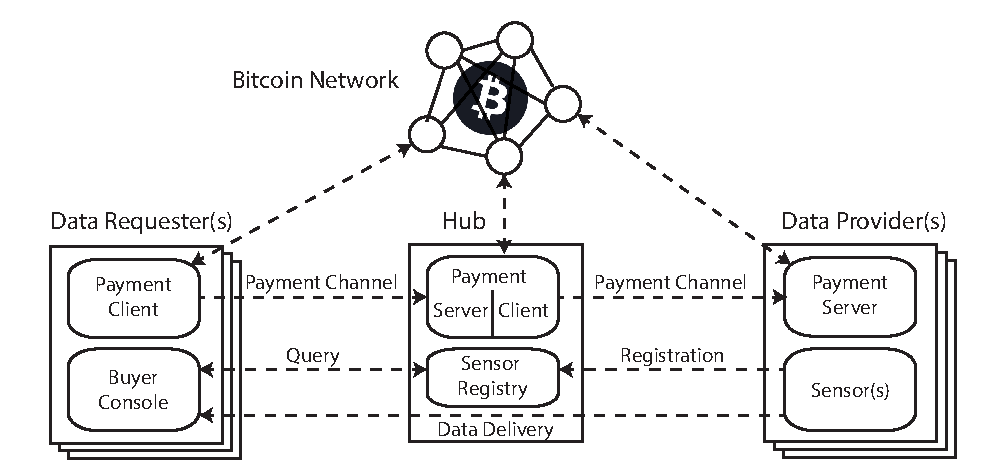
\includegraphics{Architecture.pdf}
 \caption{Overview of system's architecture.}
 \label{fig:architecture}
 \end{figure*}

\section{Prototype Implementation}
\label{sec:implementation}

The implementation of N-to-M mediated payment channels is based on extending the payment channel implementation of the bitcoinj library \cite{Bitcoinj}. Bitcoinj is a Java library for working with the Bitcoin protocol and was the first Bitcoin library that had implemented support for payment channels. The Java implementation was chosen because it allows to reuse the implementation across all of the system's components. JavaScript provides the same benefits but libraries were not as mature at that point in time. Furthermore, bitcoinj implements simplified payment verification (SPV). It allows to verify on-chain transactions without needing to store and verify the entite Bitcoin blockchain. SPV nodes store only the block headers (80 byte instead of a few hundred kilo byte for a typical block). In order to validate a particular transaction, a SPV node demands the Merkle branch that entails the transaction and is thus able to verify that the transaction is in a particular block by comparing the calculated Merkle root with the one in the stored block header. Only due to the SPV approach it is viable to use Bitcoin on resource constrained devices without trusting third party services.

The data requester and the hub are implemented as native Java applications. The data provider is implemented as an Android application. Before presenting the implementation of the individual components we start with the common building block on which all peer-to-peer payments are based. 

\subsection{Mediated payment channels using HTLCs}

We follow the client-server architecture of the payment channel implementation of bitcoinj \cite{BitcoinjPC}. A client is always on the sending side of a payment while a server is on the receiving side (c.f. Figure \ref{fig:architecture}). Since the hub acts as mediator or router for payments between requesters and providers it has to receive payments from requesters and forward those payments to providers. Hence, the hub incorporates both, server and client.

\begin{table}
  \centering
    \caption{The five layers of the HTLC payment channel implementation.}
  \begin{tabular}{|c|l|}
    \hline
    \tabhead{Layer} &
    \tabhead{Description} \\
    \hline
    Driver Application & \multicolumn{1}{|p{0.5\columnwidth}|}{Provides the API to access lower layers}\\
    \hline
    Channel Connection & \multicolumn{1}{|p{0.5\columnwidth}|}{Provides the interface to the network}\\
    \hline
    Payment Channel & \multicolumn{1}{|p{0.5\columnwidth}|}{Handles messages from/to the network and passes instructions/gets results to/from the lower layer}\\
    \hline
    Channel State Machine & \multicolumn{1}{|p{0.5\columnwidth}|}{Handles the state of the payment channel}\\\\
    \hline
    HTLC State Machines & \multicolumn{1}{|p{0.5\columnwidth}|}{Handles the state of the HTLC}\\\\
    \hline
  \end{tabular}
  \label{tbl:layers}
\end{table}

In order to implement hashed HTLCs we extended the four layers of bitcoinj's payment channel implementation with a fifth layer that is concerned with keeping track of the HTLC flow. The five layers are described briefly in Table \ref{tbl:layers}. Details about the state machines and sequence diagrams can be found in BLINDED FOR REVIEW.
Messages and transactions are serialized using Google protocol buffers\footnote{https://developers.google.com/protocol-buffers/} and are exchanged between the components over TCP connections. The payment channel setup and the HTLC payments in the implementation are slightly more complex and involve even more communication than it is shown in Table \ref{tabl:htlcflow} because we use the interactive approach for channel refunds. 

\subsection{Data provider}

The data provider is implemented as an Android application. The application allows users to offer measurement data from various sensors at an adjustable price denominated in satoshis\footnote{A satoshi is the smallest fraction of a bitcoin and corresponds to $10^{-8}$ bitcoins}. Table \ref{tbl:sensors} provides an overview of possible sensors. With the initial boot of the application, a local wallet is generated. The wallet is responsible for generating and storing key pairs and signing transactions. Furthermore a background service is started that manages the payment channel server and data delivery. If a user decides to offer measurement data from a specific sensor, the application registers the sensor at the global sensor registry. The initial registration then triggers the setup of a payment channel between the hub and the Android application. As soon as the payment channel is established the application is ready to serve requests from buyers.


\begin{table}
  \centering
  \caption{Examples of virtual and physical sensors available in smartphones.}
  \begin{tabular}{|c|l|l|}
    \hline
    \tabhead{Sensor} &
    \tabhead{Type} &
    \tabhead{Application} \\
    \hline
    Barometric pressure & physical & Weather prediction \\
    \hline
    Location & both & People flow  \\
    \hline
    Network strength & physical & Coverage maps \\
    \hline
    Installed apps & virtual & Inter-app correlations    \\
    \hline
    Transportation mode & virtual & City monitoring \\
    \hline
    Steps & virtual & Health monitoring  \\
    \hline
  \end{tabular}
  \label{tbl:sensors}
\end{table}


\subsection{Data requester}
The data requester is implemented as a Java application. The requester application allows to query the sensor registry. In the prototype this is achieved using simple console commands. Table \ref{tbl:commands} shows the available commands.

\begin{table}
  \centering
    \caption{Available commands of the data requester console.}
  \begin{tabular}{|c|l|}
    \hline
    \tabhead{Command} &
    \tabhead{Description} \\
    \hline
    STATS NODES & Returns all connected sensor nodes \\
    \hline
    STATS SENSORS & Returns available sensor types \\
    \hline
    SELECT SENSOR=$<$type$>$ & \multicolumn{1}{|p{0.5\columnwidth}|}{Returns sensors of type $<$type$>$ with pricing information} \\
    \hline
    BUY $<$type$>$ FROM $<$node$>$ & \multicolumn{1}{|p{0.5\columnwidth}|}{Buys the current measurement value of sensor $<$type$>$ from node $<$node$>$} \\
    \hline
   
    \hline
  \end{tabular}
  \label{tbl:commands}
\end{table}



\subsection{Hub}
The hub acts as the central point of coordination. Data providers register their sensors with the sensor registry that the hub provides, and data requesters are able to query the registry. Furthermore, the hub is responsible for mediating the payments between buyers and sellers. The hub instantiates a payment channel client and a payment channel server





\section{Evaluation}

\subsection{Conceptual Evaluation}

\subsubsection{Low barrier for participation}
A potential participant on the data provider side has to download and install the data provider smartphone application. The data provider does not need to own any bitcoins. Furthermore no manual sign-up or registration is required. This means also the system has global reach and could provide a low-income stream to smartphone users in developing countries.

A data requester does not have to register but the wallet of the data requester application needs to have some amount of bitcoin in order to initiate a payment channel with the hub.

\subsubsection{Incentivize participation with micropayments}
Individual payments can be as low as 1 satoshi. In April 2015, the exchange rate is around 450\$/BTC. In regard to this exchange rate individual payments can be as low as 4.5 $\mu$\$. Even smaller payments could be implemented with probabilistic payment schemes \cite{Rivest1997,Pass:2015:MDC:2810103.2813713}. Transaction fees for setting up and closing payment channels will be discussed in Sec. \ref{sec:fees}. 

\subsubsection{Limited trust in hub provider}
The usage of HTLCs to interconnect payment channels of data providers and data requesters allows atomic payments between those parties. This means either the payment happens in both channels or it happens not at all. 

\subsubsection{Anonymity}
Obviously there is a risk of de-anonymization for data providers depending on the data they are selling. However we restrict the evaluation of anonymity to the payment aspect. Bitcoin payments themselves are pseudonymous. Transactions only entail cryptographic public keys and hashes thereof. Thus, if a user is careful, Bitcoin provides a high level of anonymity. In addition, due to the usage of mediated payment channels, there is no public link between buyers and sellers. Only transactions between buyers and the hub, and sellers and the hub end up in the blockchain. Most of the transactions entailing the linking secret are kept private. Only if a payment channel has to be closed before its capacity is depleted a revealing transaction ends up in the Bitcoin blockchain.

In addition, there is a risk of de-anonymization based on the IP addresses. However since all communications are based on TCP, it would be possibly to run the system over Tor\footnote{https://www.torproject.org/}.


\subsection{Empirical Evaluation}

\subsection{Performance}

For setting up and closing of payment channels the Bitcoin network itself is dictating the performance. If fees are sufficient a transaction can be assumed to be included in the blockchain in 10 min on average. Depending on the value of the transaction the receiver of the funds might wait until the transaction has six confirmations. This means that there are five additional blocks on top of the block entailing the transaction. 
In the following we assume that payment channels are already in place and evaluate the time is takes to complete a payment. The experiment was done by instantiating 100 data requesters and one data provider. Each requester buys one measurement value from the data provider. Table \ref{tbl:performance} shows a breakdown of the mean times and the standard deviation according to the payment steps. The results request some explanation. First, the HTLC setup process between hub and provider seems to take almost twice as long as the the HTLC setup between requester and hub. The reason for this is that the hub-provider setup is initiated with generating the secret but then has to wait until requester-hub setup is finished. If the hub would initiate the HTLC setup with the provider immediately the hub would risk paying the provider without being pull the respective funds from the requester. Second, the teardown (i.e. updating the setup transacting by assigning the value of HTLC output to the payee.) process takes less than half the time of the setup process. The reason for that is mainly that in the actual implementation the interactive refund approach was used. This means that there is an additional transaction which has to be signed by both parties and has to be transferred from payer to payee and back. Thus, we expect a comparable performance between setup and teardown if the non-interactive approach is used. Furthermore, we see that the steps that involve the provider take more time. This is because signing and signature verification are computation intensive tasks and the data provider is a comparably weak smartphone.

\begin{table}
\centering
\caption{Payemt duration breakdown}
\begin{tabular}{|l|r|r|}
\hline
{\bf Payment } & \multicolumn{1}{l|}{{\bf Mean}} & \multicolumn{1}{l|}{{\bf St. Dev.}} \\ \hline
Requester-Hub setup             & 479.3 ms                 & 78.8 ms                      \\ \hline
Hub-Provider setup            & 1015.1 ms                & 151.4 ms                     \\ \hline
Hub-Provider teardown         & 199.6 ms                 & 68.3 ms                      \\ \hline
Buyer-Provider teardown          & 146.6 ms                 & 10.1 ms                      \\ \hline
\end{tabular}

\label{tbl:performance}
\end{table} 


\subsection{Transaction costs}
\label{sec:fees}
Transaction fees in Bitcoin are in principle voluntary. The party that creates a transaction specifies the transaction fees as the difference of the sum of the value of all inputs and the sum of the value of all outputs. However, each miner can decide individually if she will accept the transaction for a candidate block. Since there is a limit on the maximum size of a block, and larger blocks need more time to propagate the network, rational miners will select transactions with higher transaction fees. This is also the reason why transaction fees are based on the size of the transaction instead of its value. The transaction size is mainly defined by the number and size of input and output scripts and signatures. Figure \ref{fig:tx_fees} shows the daily averages of transaction fees in USD/kb for the period of one year.

\begin{figure}[!t]
\centering
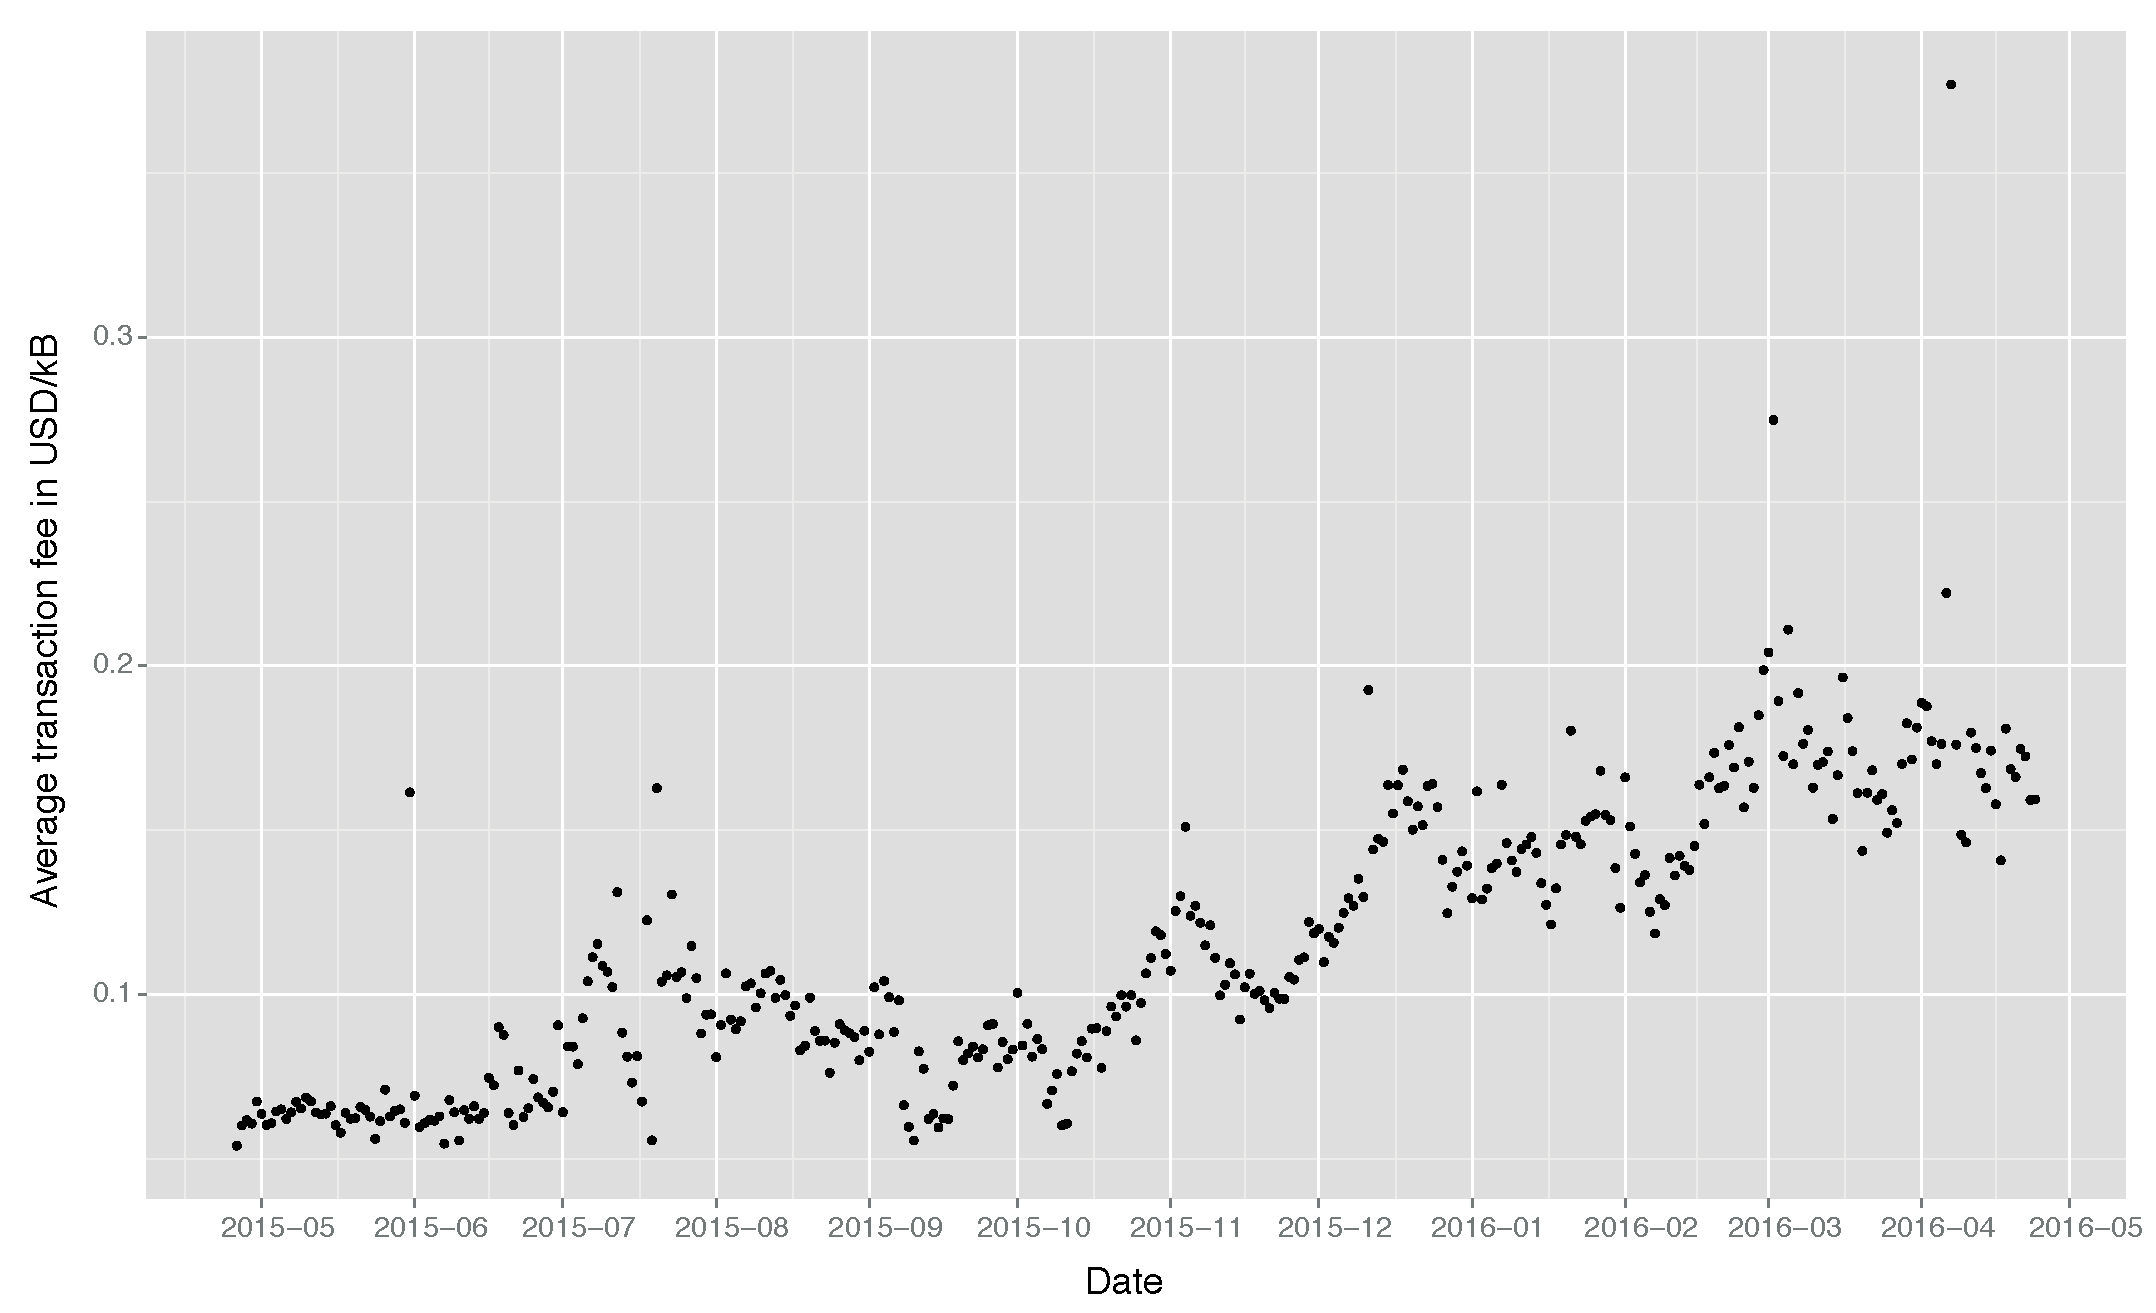
\includegraphics[width=\linewidth]{fees_per_kb}
\caption{Bitcoin transaction fees in USD/kb. Each point represents a daily average.}
\label{fig:tx_fees}
\end{figure}


\begin{table}
  \centering
  \caption{Approximate sizes and costs for Bitcoin transactions}
  \begin{tabular}{|c|l|l|}
    \hline
    \tabhead{Transaction Type} &
    \tabhead{Size} &
    \tabhead{Cost} \\
    \hline
    Standard P2PKH & \multicolumn{1}{|p{0.5\columnwidth}|}{} & \\
    \hline
    Funding & \multicolumn{1}{|p{0.5\columnwidth}|}{} & \\
    \hline
    HTLC setup & \multicolumn{1}{|p{0.5\columnwidth}|}{} & \\
    \hline
    Settlement & \multicolumn{1}{|p{0.5\columnwidth}|}{} & \\
    \hline
    Forfeiture & \multicolumn{1}{|p{0.5\columnwidth}|}{} & \\
    \hline
  \end{tabular}
  \label{tbl:fees}
\end{table}


\section{Discussion}

\subsection{Intermittent connectivity}
In order for the payment mechanism to be trustless payment receivers 


\subsection{Locking of funds}

The usage of payment channels involves locking of funds. This is a problem in particular for the payment hub. One of our principles was that the onboarding of new data producers should be frictionless. Hence, we assume that data producers do not have any bitcoins to begin with. When a data producer registers a sensor with the registry the payment hub initiates a payment channel with the data producer. As described in Sec. \ref{sec:mediated} this involves broadcasting a funding transaction to the Bitcoin network. Thereby the hub has to lock capital in the channel and has to provide a fee in order for the transaction to be mined. The operator has to balance between locking a large amount and the transaction costs involved in closing and reopening a channel because of depletion.
Since there is no cost for a data producer to register, a malicious actor might attack the hub by registering a large amount of fake sensors. A strategy to disincentive such a behavior would be to request proof of work from the sensor as part of the registration process. 
In addition the locking of funds is a problem for benevolent data requesters since the earned satoshis are only usable for payments after closing of the channel. 


\subsection{Improving anonymity}



\subsection{Discovery}

\subsection{From smartphones to wireless sensor networks}

\subsubsection{Additional challenges}
% An example of a floating figure using the graphicx package.
% Note that \label must occur AFTER (or within) \caption.
% For figures, \caption should occur after the \includegraphics.
% Note that IEEEtran v1.7 and later has special internal code that
% is designed to preserve the operation of \label within \caption
% even when the captionsoff option is in effect. However, because
% of issues like this, it may be the safest practice to put all your
% \label just after \caption rather than within \caption{}.
%
% Reminder: the "draftcls" or "draftclsnofoot", not "draft", class
% option should be used if it is desired that the figures are to be
% displayed while in draft mode.
%
%\begin{figure}[!t]
%\centering
%\includegraphics[width=2.5in]{myfigure}
% where an .eps filename suffix will be assumed under latex, 
% and a .pdf suffix will be assumed for pdflatex; or what has been declared
% via \DeclareGraphicsExtensions.
%\caption{Simulation results for the network.}
%\label{fig_sim}
%\end{figure}

% Note that the IEEE typically puts floats only at the top, even when this
% results in a large percentage of a column being occupied by floats.
% However, the Computer Society has been known to put floats at the bottom.


% An example of a double column floating figure using two subfigures.
% (The subfig.sty package must be loaded for this to work.)
% The subfigure \label commands are set within each subfloat command,
% and the \label for the overall figure must come after \caption.
% \hfil is used as a separator to get equal spacing.
% Watch out that the combined width of all the subfigures on a 
% line do not exceed the text width or a line break will occur.
%
%\begin{figure*}[!t]
%\centering
%\subfloat[Case I]{\includegraphics[width=2.5in]{box}%
%\label{fig_first_case}}
%\hfil
%\subfloat[Case II]{\includegraphics[width=2.5in]{box}%
%\label{fig_second_case}}
%\caption{Simulation results for the network.}
%\label{fig_sim}
%\end{figure*}
%
% Note that often IEEE papers with subfigures do not employ subfigure
% captions (using the optional argument to \subfloat[]), but instead will
% reference/describe all of them (a), (b), etc., within the main caption.
% Be aware that for subfig.sty to generate the (a), (b), etc., subfigure
% labels, the optional argument to \subfloat must be present. If a
% subcaption is not desired, just leave its contents blank,
% e.g., \subfloat[].


% An example of a floating table. Note that, for IEEE style tables, the
% \caption command should come BEFORE the table and, given that table
% captions serve much like titles, are usually capitalized except for words
% such as a, an, and, as, at, but, by, for, in, nor, of, on, or, the, to
% and up, which are usually not capitalized unless they are the first or
% last word of the caption. Table text will default to \footnotesize as
% the IEEE normally uses this smaller font for tables.
% The \label must come after \caption as always.
%
%\begin{table}[!t]
%% increase table row spacing, adjust to taste
%\renewcommand{\arraystretch}{1.3}
% if using array.sty, it might be a good idea to tweak the value of
% \extrarowheight as needed to properly center the text within the cells
%\caption{An Example of a Table}
%\label{table_example}
%\centering
%% Some packages, such as MDW tools, offer better commands for making tables
%% than the plain LaTeX2e tabular which is used here.
%\begin{tabular}{|c||c|}
%\hline
%One & Two\\
%\hline
%Three & Four\\
%\hline
%\end{tabular}
%\end{table}


% Note that the IEEE does not put floats in the very first column
% - or typically anywhere on the first page for that matter. Also,
% in-text middle ("here") positioning is typically not used, but it
% is allowed and encouraged for Computer Society conferences (but
% not Computer Society journals). Most IEEE journals/conferences use
% top floats exclusively. 
% Note that, LaTeX2e, unlike IEEE journals/conferences, places
% footnotes above bottom floats. This can be corrected via the
% \fnbelowfloat command of the stfloats package.




\section{Conclusion}
The conclusion goes here.





% if have a single appendix:
%\appendix[Proof of the Zonklar Equations]
% or
%\appendix  % for no appendix heading
% do not use \section anymore after \appendix, only \section*
% is possibly needed

% use appendices with more than one appendix
% then use \section to start each appendix
% you must declare a \section before using any
% \subsection or using \label (\appendices by itself
% starts a section numbered zero.)
%


\appendices
\section{Refund Transactions and Time locks}
\label{app:timelock}

There are two ways to allow the payment channel creator to retrieve her funds after a specific \emph{locktime} if the payee is not cooperative. The first, an interactive method, has been available in Bitcoin for a long time. The second, a non-interactive method, has only been available since December 2015. The non-interactive methods using the \emph{CHECKLOCKTIMEVERIFY} operator provides various advantages. Thus we present the payment channels in terms of this operator although our implementation is based on the interactive approach since at time of the implementation \emph{CHECKLOCKTIMEVERIFY} was not available. For that reason we briefly present the interactive method.

Bitcoin transactions provide a data field that allows to specify a locktime in terms of a block number or an UTC timestamp. The locktime prevents a transaction to enter the blockchain before that event. This feature can be used to create a refund transaction that can spent the 2-of-2 multisignature output of the funding transaction after some time. It is important to note that the refund transaction has to be signed by the payee before the funding transaction is broadcasted to the Bitcoin network. Otherwise the payee would be able to refuse signing the refund transaction and hence the funds could be locked forever. After the payee has signed the refund transaction, the payer has to store the transaction in order to be able to retrieve the funds after the event specified with the locktime.
% you can choose not to have a title for an appendix
% if you want by leaving the argument blank
\section{}
Appendix two text goes here.


% use section* for acknowledgment
\ifCLASSOPTIONcompsoc
  % The Computer Society usually uses the plural form
  \section*{Acknowledgments}
\else
  % regular IEEE prefers the singular form
  \section*{Acknowledgment}
\fi


The authors would like to thank...


% Can use something like this to put references on a page
% by themselves when using endfloat and the captionsoff option.
\ifCLASSOPTIONcaptionsoff
  \newpage
\fi



% trigger a \newpage just before the given reference
% number - used to balance the columns on the last page
% adjust value as needed - may need to be readjusted if
% the document is modified later
%\IEEEtriggeratref{8}
% The "triggered" command can be changed if desired:
%\IEEEtriggercmd{\enlargethispage{-5in}}

% references section

% can use a bibliography generated by BibTeX as a .bbl file
% BibTeX documentation can be easily obtained at:
% http://mirror.ctan.org/biblio/bibtex/contrib/doc/
% The IEEEtran BibTeX style support page is at:
% http://www.michaelshell.org/tex/ieeetran/bibtex/
\bibliographystyle{IEEEtran}
% argument is your BibTeX string definitions and bibliography database(s)
\bibliography{IEEEabrv,crowdsensing}
%\bibliography{crowdsensing}
%
% <OR> manually copy in the resultant .bbl file
% set second argument of \begin to the number of references
% (used to reserve space for the reference number labels box)


% biography section
% 
% If you have an EPS/PDF photo (graphicx package needed) extra braces are
% needed around the contents of the optional argument to biography to prevent
% the LaTeX parser from getting confused when it sees the complicated
% \includegraphics command within an optional argument. (You could create
% your own custom macro containing the \includegraphics command to make things
% simpler here.)
%\begin{IEEEbiography}[{\includegraphics[width=1in,height=1.25in,clip,keepaspectratio]{mshell}}]{Michael Shell}
% or if you just want to reserve a space for a photo:

\begin{IEEEbiography}{Michael Shell}
Biography text here.
\end{IEEEbiography}

% if you will not have a photo at all:
\begin{IEEEbiographynophoto}{John Doe}
Biography text here.
\end{IEEEbiographynophoto}

% insert where needed to balance the two columns on the last page with
% biographies
%\newpage

\begin{IEEEbiographynophoto}{Jane Doe}
Biography text here.
\end{IEEEbiographynophoto}

% You can push biographies down or up by placing
% a \vfill before or after them. The appropriate
% use of \vfill depends on what kind of text is
% on the last page and whether or not the columns
% are being equalized.

%\vfill

% Can be used to pull up biographies so that the bottom of the last one
% is flush with the other column.
%\enlargethispage{-5in}



% that's all folks
\end{document}


